%  Formatting the Paper  -------------------------------------------------------
\documentclass[a4paper,11pt]{report}

% adjust margins
\usepackage[right=1in,top=1in,left=1in,bottom=1in]{geometry}


%  Packages Used  --------------------------------------------------------------
% graphics (images)
%\usepackage{graphicx}
\usepackage[english]{babel}
\usepackage[pdftex]{color,graphicx}


%  Start the Paper  ------------------------------------------------------------
% define the title
\title{Project 1 - Any Angle Path}
\author{Qandeel Sajid and Tina Nye}
\begin{document}
\maketitle

% insert the table of contents
\newpage
\tableofcontents
\newpage

\section{Project Description}
Path Planning is an important aspect of artificial intelligence that can be used for multiple applications especially in the field of robotics and computer gaming. In gaming, good path planning makes the difference in the quality of games; it is likely that the player has to navigate on a grid while avoiding obstacles and looking for the shortest path to its desired destination. To find the shortest path, path planning depends heavily on search algorithms that can find the best path under time and space constraints. Some of these search algorithms include A*, Theta* or using the Visibility Graphs to search the grid.

In this assignment, the focus is to implement A* and Theta*. This paper discusses the implementation of these algorithms and tested them on 50 different randomly generated grid samples. A* on a grid, Theta*, and A* on a visibility graph are tested on the same 50 grids. This paper discusses the results and compares the algorithms based on the path costs and runtimes. After the discussion, solutions to the problems given for this project are shown.
 
\section{Implementation}
The program for this project is done in Python, and the visualization is implemented with PyGame. For the program, the standard size of the grid is 100 columns by 50 rows. The grid size can be altered by changing the values of the variables \textit{colLength} and \textit{rowLength} found above in the files functions.py and main.py. The graph and visualization are called in main.py. A* and Theta* are abstracted into a class which, when called by the main, return the path found. More details on the implementation are found below.
	\subsection{Graph Setup}
	The graph for the program is implemented using SparseGraph from the Python standard graph library. Each end of a cell on the grid represents a vertex in the graph. The blocked cells are visualized by the gray cells. These vertices are connected to neighboring vertices through an edge if that edge does not go through a blocked cell. Additional functions found in functions.py are used to convert between the vertex ID, and the pixel location of the vertex. Figure~\ref{fig:graph_image} shows the connected edges highlighted in red. The surrounding gray cells represent a border around the grid.
	
	For the implementation of the graph, only the top-left (x, y) value is remembered for the obstacles. This will be important later in the report for the implementation of Theta*.

	
	%% show the graph image
	\begin{figure}[h!]
	  \centering
	    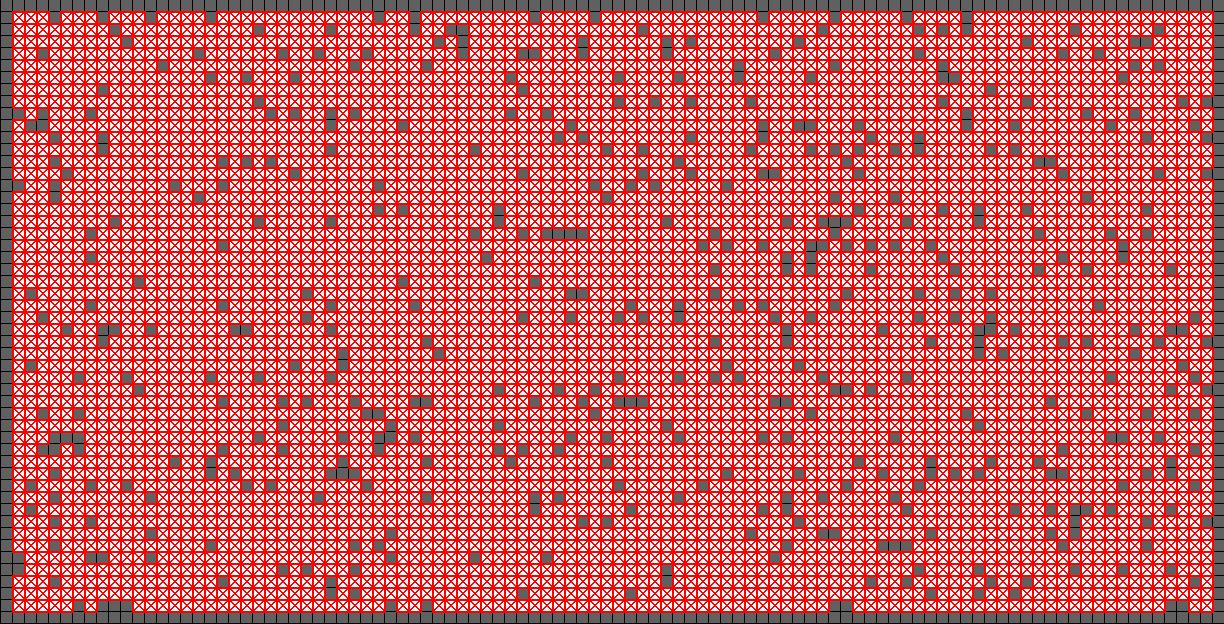
\includegraphics[width=1\textwidth]{images/graph.png}
	  \caption{Visualization of the graph used by the program}
	  \label{fig:graph_image}
	\end{figure}
	%%%%%%
	
	\subsection {A*}
	Figure~\ref{fig:ai_algorithm} shows the pseudo-code for the A* algorithm used in the implementation. The actual implementation of the code follows the pseudo-code closely. Originally, the implementation of A* used the standard binary heap that comes with Python as the fringe. The fringe ordered the nodes so the one with the smallest f(n) value is on top. It broke ties using the total path cost (g(n)). After the first demo of the project, we implemented our own binary heap using Python lists. 
	
	Optimization was our goal for the first implementation of A*. For optimization there is no specific list for the "closed" vertices. Instead, flags for whether the vertex is in the fringe or has been expanded are stored in the vertex of the graph. By doing this, the algorithm did not not require looping through the set of vertices in the closed list; it would know if the node has been expanded as soon as it checks the boolean value for that vertex from the graph.
	Something done to optimize the first implementation of the algorithm is that the algorithm does not have to check for blocked cells as it is planning. Only valid edges have been inserted into the graph which means A* never has to test whether an edge between two vertices is through a blocked cell. The results show this gives a faster solution.
	After the demo, another optimization was done through the binary heap. For the standard binary heap there was no way to remove a vertex so the authors implemented their own. The remove function required copying all the elements, except the one that has to be removed, into a new heap. Obviously, this is wasteful since it requires a hard copy of the of the heap every time a node needed to be removed. The new implementation uses the remove function for Python lists.
	
	%% show the A* algorithms
	\begin{figure}[h!]
	    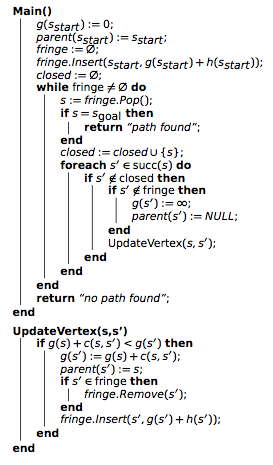
\includegraphics[width=.45\textwidth]{images/ai_algorithm.png}
	  \caption{Shows the pseudo-code for the A* algorithm used in the implementation}
	  \label{fig:ai_algorithm}
	\end{figure}
	%%%%%%
	
	\subsection{Theta*}
	Theta* allows paths to go through cells rather than just moving from corner to corner on the cell as well as connect to vertices that are not neighbors. This gives better-looking, shorter paths for games. The main parts of the Theta* algorithm are similar to A*. The difference lies with the UpdateVertex function shown in Fig.~\ref{fig:theta_algorithm}. As shown, this algorithm relies on the use of the LineOfSight function. The project was provided with an algorithm for implementing the LineOfSight which just checks if the straight line connection between two vertices does not go through any blocked cells. Unfortunately, with the way the authors implemented the graph (remembering only the top-left (x, y) values of the obstacles cells), the algorithm given for LineOfSight cannot be used in this project. For this, the authors made a customized function that does the same thing as LineOfSight. This function just finds a linear equation to represent the straight line connecting between the two points. Then, in small intervals, the functions checks the (x, y) value from the equation and rounds the value down to check if the (x, y) values matches top-left x,y value of an obstacle. 
	
	After the first demo, the authors discovered two bugs in the program. One of the bugs occurred very rarely but has to do with how the function check of the floored (x, y) value matched that of an obstacle. The second bug had to do with the interval at which the function is checked. On a grid with larger cells, the interval can be large as well. For smaller cell the interval also needs to be small otherwise it mistakenly gives a wrong solution in which paths go through blocked cells. By having a smaller interval, the function takes longer to check if a path is free. Smaller intervals are not done in original Theta* causing the time taken by the optimized to be similar to the original.  Theta* was optimized the same way as A*.

	%% show the Theta* algorithms
	\begin{figure}[h!]
	    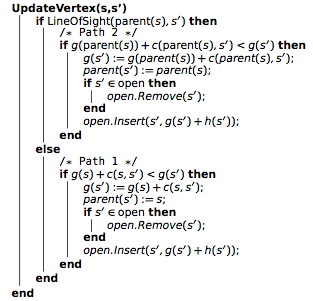
\includegraphics[width=.5\textwidth]{images/theta_algorithm.png}
	  \caption{Shows the pseudo-code for the Theta* algorithm used in the implementation}
	  \label{fig:theta_algorithm}
	\end{figure}
	%%%%%%	

	\subsection{Visibility Graph}
	In the Visibility Graph, only edges connecting the corner of blocked cells are allowed. These edges cannot go through any blocked vertices. The Visibility Graph is made by iterating through the corners of the obstacles and checking if the edge is free of obstacles using LineOfSight. Then A* is just applied to the Visibility Graph to find the shortest path from the start to goal. The algorithm for the Visibility Graph is not shown. 

\section{Results and Discussion}
Both the original A* and Theta* and their optimized versions were run on the same set of 50 randomly generated grids with only 10 percent of the cells as obstacles. Lastly, the Visibility Graph was run on that same set of 50 grids. The results are shown and discussed below.  These tests were conducted on a machine with an Intel core i7 CPU and an nVidia GeForce GTX 560M.
%-------------------------------------------------------------------------------
\subsection{Original A* and Theta*}
Tables~\ref{table:original_path_lengths} and ~\ref{table:original_runtimes} show the average path lengths and runtimes found by running the set of 50 grids mentioned above when 10 percent and 50 percent of the cells as obstacles respectively. As shown by the path lengths results, Theta* gives the shorter path. This is definitely because Theta* can move to vertices that are not its direct neighbors.

% table for original implementation results -- path length
\begin{table}[h!]
   \centering
   \begin{tabular}{ | c | c | c | }

      \hline
      \textbf{100x50 Grid} & \textbf{A* on Grid} & \textbf{Theta*}  \\ \hline
      Random Obstacles, 10\% & 43.5766 & 41.394  \\ \hline
      Random Obstacles, 50\% & 45.2565 & 42.8329  \\ \hline
   \end{tabular}

   \caption{Path length}
   \label{table:original_path_lengths}
\end{table}

Although the Theta* algorithm has to traverse each edge it finds using the LineOfSight function, it still takes less time than the A* algorithms. This is likely because the path it finds, although shorter than A*, might not be as short as it could have been. Theta* also does not have to waste time looking at just its closest neighboring vertices, it can jump to an vertex that it can reach with a valid edge. In addition, this implementation of Theta* uses larger intervals to check the linear equation in the LineOfSight which gives it a lot smaller runtime than expected.

As shown by the Tables, the algorithms clearly give a long path and take more time for their solution when the percentage of obstacles is at 50.

% table for original implementation results -- runtime
\begin{table}[h!]
   \centering
   \begin{tabular}{ | c | c |c | }

      \hline
      \textbf{100x50 Grid} & \textbf{A* on Grid} & \textbf{Theta*}   \\ \hline
      Random Obstacles, 10\% & 31.187 & 8.93683  \\ \hline
      Random Obstacles, 50\% & 34.4797 & 9.74801  \\ \hline

   \end{tabular}

   \caption{Runtime}
   \label{table:original_runtimes}
\end{table}


%-------------------------------------------------------------------------------
\subsection{Optimized A* and Theta*}
The optimized versions of A* and Theta* were tested on the same set of 50 randomly generated grid as their original counterparts. The results are shown in Tables~\ref{table:optimized_path_lengths} and ~\ref{table:optimized_runtimes}. Due to a lack of time, these algorithm were not tested on grids with 50 percent algorithms. In the optimized, the paths found by the Theta* are not noticeably better than those found by A*, but they still are shorter. The time taken by Theta* to find the solution is more than the A*. As mentioned above, the optimized Theta* uses smaller intervals in its LineOfSight equation which causes it to take more time than the optimized A* compared to how well the originals did. 

% table for optimized implementation results -- path length
\begin{table}[h!]
   \centering
   \begin{tabular}{ | c | c |c |c | }

      \hline
      \textbf{100x50 Grid} & \textbf{A* on Grid} & \textbf{Theta*}  \\ \hline
      Random Obstacles, 10\% & 40.9819 & 39.2298\\ \hline
      Random Obstacles, 50\% & N/A & N/A \\ \hline

   \end{tabular}

   \caption{Path length}
   \label{table:optimized_path_lengths}
\end{table}


% table for optimized implementation results -- runtime
\begin{table}[h!]
   \centering
   \begin{tabular}{ | c | c |c |c | }

      \hline
      \textbf{100x50 Grid} & \textbf{A* on Grid} & \textbf{Theta*} \\ \hline
      Random Obstacles, 10\% & 27.3734 & 34.7868  \\ \hline
      Random Obstacles, 50\% & N/A & N/A \\ \hline

   \end{tabular}

   \caption{Runtime}
   \label{table:optimized_runtimes}
\end{table}


%-------------------------------------------------------------------------------
\subsection{Comparison between old and new implementation results}
The averaged path length found by the original A* compared to the optimized is about 5 percent longer and the same can be said for the Theta* implementations. The focus of the optimization is actually not the path length since nothing that can radically affect the path lengths was implemented in the optimized version. 

The optimization was for improving the runtime found by both algorithms. As shown by the tables above, the averaged runtime for optimized A* is about 20 percent less than that taken by the original. This is likely because of the efficient implementation of the binary heap remove. By not hard copying the heap, the optimized decreased in the amount of time it takes. 
The results given Theta* cannot be objectively compared. The optimized version of Theta* uses smaller intervals while the original uses larger to check edges.

\subsection{Visibility Graph}
Tables~\ref{table:visibility_path_lengths} and ~\ref{table:visibility_runtimes} show the path length and runtime taken for the same set of 50 grids. The average path found by applying A* on a Visibility Graph is better those found by either implementation of Theta*. This is because the Visibility Graph connects only the useful edges (those around obstacles) compared to Theta* which just connect to vertices with low f(n) values. 


\begin{table}[h!]
   \centering
   \begin{tabular}{ | c | c |c |c | }

      \hline
      \textbf{100x50 Grid} & \textbf{A* on Visibility Graph}  \\ \hline
      Random Obstacles, 10\% & 39.1003 \\ \hline
      Random Obstacles, 50\% & N/A  \\ \hline

   \end{tabular}

   \caption{Path length}
   \label{table:visibility_path_lengths}
\end{table}

The time taken by the Visibility Graph is horrible though because iterating through edges and applying LineOfSight takes a long time in Python. To reduce the time taken by the algorithm, only nodes being expanded connect to the vet ices in the graph.

\begin{table}[h!]
   \centering
   \begin{tabular}{ | c | c |c |c | }

      \hline
      \textbf{100x50 Grid} & \textbf{A* on Visibility Graph}  \\ \hline
      Random Obstacles, 10\% & 1376.18  \\ \hline
      Random Obstacles, 50\% &  N/A  \\ \hline

   \end{tabular}

   \caption{Runtime}
   \label{table:visibility_runtimes}
\end{table}


%-------------------------------------------------------------------------------
\section{A* heuristic vs Theta* heuristic}

From the results in Table 1 and Table 3, Theta* always has shorter path lenths; however, A* and Theta* switched between which one was faster depending on the implementation as seen in Table 2 and Table 4.  This discrepancy in runtimes may be due to the non-monotonic property of Theta*; it is able to find a shorter path at the expense of runtime.  Otherwise, the discrepancy may be due to something that might have happened/changed in the optimized implementation.

On a grid, it is fair that A* and Theta* use different h-values.  A* can only traverse along edges, which in the case of a grid, is eight discrete directions, but Theta* can traverse a path in a direction along any angle.  It makes sense that Theta* uses the striaght-line (linear) distance formula between two points to calculate the its heuristic because it can move in any angle, so since A* does not have this capability it needs a heuristic that gives a appropriate distance from the goal while considering its movement capabilities.  According to A. Nash et al. in the paper "Theta*: Any-Angle Path Planning on Grids", "A* with consistent h-values finds paths of the same length no matter how small or large the h-values are."  In conclusion, it is a legitimate arguement that A* and Theta* use different h-values.



%-------------------------------------------------------------------------------
\section{Explain why A* with the h-values from Equation 1 is guaranteed to find shortest grid paths}
Equation 1 calculates the Manhattan distance, which is the sum of all hoizontal and vertical distances from the current vertex to the goal.  By using the Manhattan distance as a heuristic function, A* never overestimates the distance to the goal, thus making it admissible.  This does not consider if there are obstacles in the path that could make the path longer; therefore, it assumes the shortest path along eight discrete directions.  A* is also consistent (or monotonic) because a node selected for expansion was reached because it had the lowest possible cost.  This is similar to Dijkstra's best-first search algorithm to find the shortes path in a graph with no negative edges.  The monotonic property of A* is that the f-value of an expanded vertex can not be any larger than one of its unexpanded visible neighbors after updating the nodes.  Which means that any expanded vertex that traverses in reverse following the parents will yeild the shortest path from the start vertex to the expanded vertex in reverse.  As a result, A* is guaranteed to find the shortest grid paths with the h-values from Equation 1 because it is admissible and consistent (monotonic).

%-------------------------------------------------------------------------------
\section{Admissibility vs Monotonicity}

Unlike the monotonic property of A*, Theta* can have an expanded vertex with an f-value larger than an f-value of one or more of its unexpanded visible neighbors.  Consequently, any expanded vertex that traverses in reverse following the parents is not guaranteed to yeild the shortest path from the start vertex to the expanded vertex in reverse.  This implies that Theta* has the ability find shorter paths at the expense of the runtime by expanding verticies more than once, whereas A* cannot.  Figure~\ref{fig:non-monotonic_theta} shows an example of the non-monotonicity of Theta*: Start vertex C1 expands to vertex B2, sets $f(B2) = 1.41+3.16 = 4.57$, and sets the parent of B1 to C1.  Then, Theta* expands vertex B2 to vertex B3, sets $f(B3) = 2.24+2.24 = 4.48$, and sets the parent of B3 to B2.  Under these circumstances, the expanded vertex B2 has a larger f-value than its unexpanded visible neighbor B3.

% display figure
\begin{figure}[h!]
  \centering
    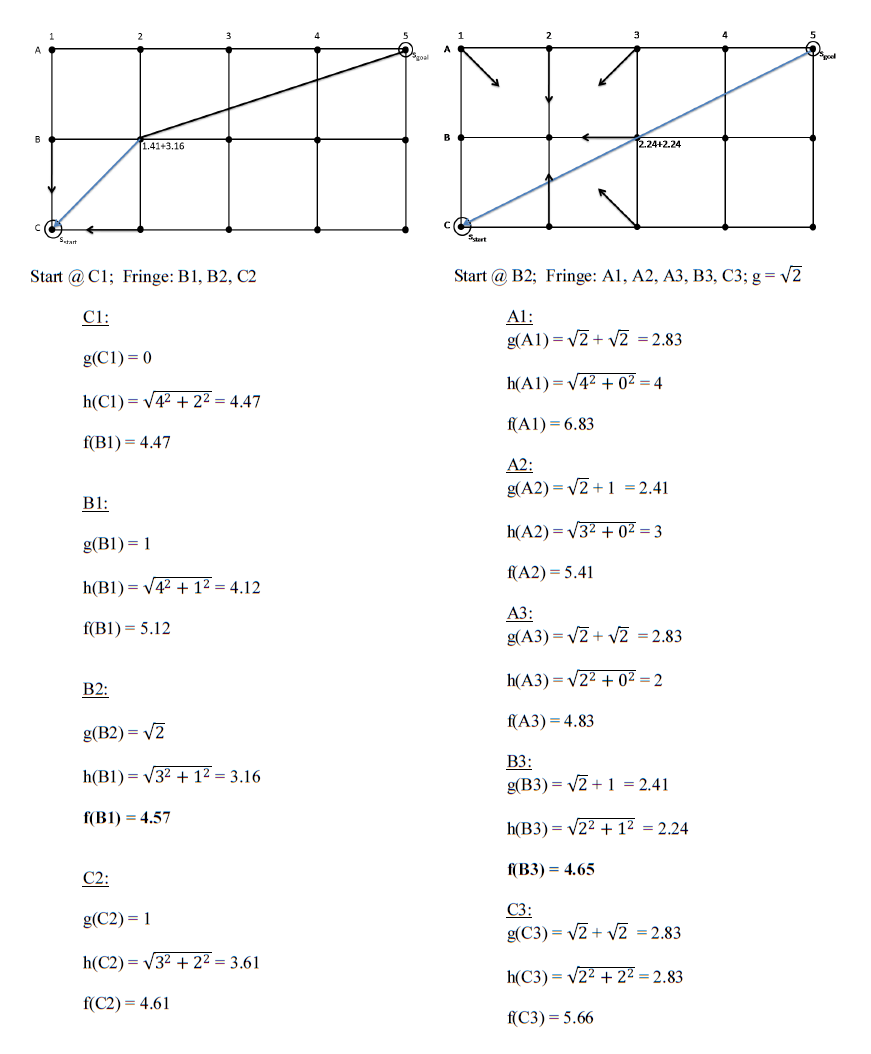
\includegraphics[width=1.0\textwidth]{part_i.png}
  \caption{Theta* non-monotonic f-values}
  \label{fig:non-monotonic_theta}
\end{figure}

\end{document}
